\begin{frame}
\frametitle{Recaudo acumulado (Ene–May)}
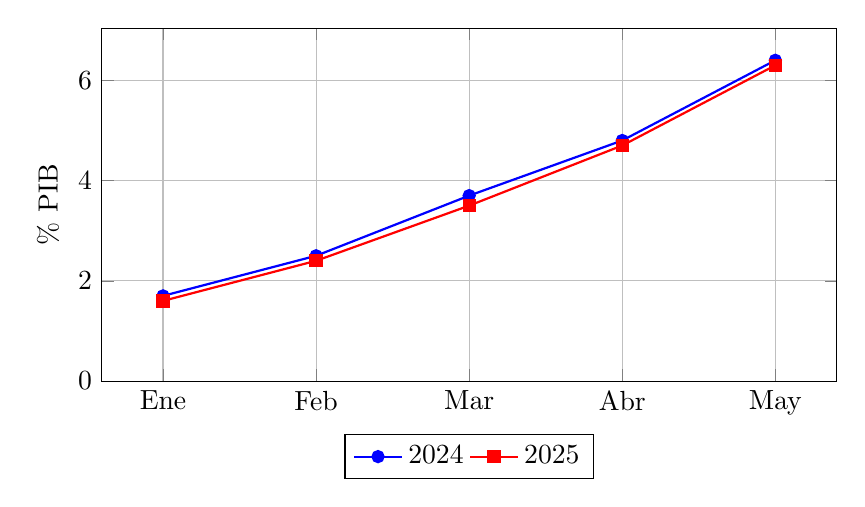
\begin{tikzpicture}
\begin{axis}[
    width=0.9\textwidth,
    height=0.5\textwidth,
%    xlabel={Mes},
    ylabel={\% PIB},
    xtick={1,2,3,4,5},
    xticklabels={Ene,Feb,Mar,Abr,May},
    grid=both,
    legend style={at={(0.5,-0.15)}, anchor=north, legend columns=-1},
    ymin=0
]

% Datos 2024
\addplot[
    thick,
    mark=*,
    color=blue
] coordinates {
    (1,1.7) (2,2.5) (3,3.7) (4,4.8) (5,6.4)
};
\addlegendentry{2024}

% Datos 2025
\addplot[
    thick,
    mark=square*,
    color=red
] coordinates {
    (1,1.6) (2,2.4) (3,3.5) (4,4.7) (5,6.3)
};
\addlegendentry{2025}

\end{axis}
\end{tikzpicture}
\end{frame}
